\subsection{Autoregressive logistic model}\label{sec:autorregresivo}

An autoregressive model explains the present value of a series from its own
past values. In its classical form, AR($p$), the observation $y_t$ is a
linear combination of the $p$ lags $y_{t-1},\dots,y_{t-p}$ plus noise. Here
the response is binary (exceedance day or not), so temporal dependence cannot
enter as a linear mean; it enters as a term in the linear predictor of a
logistic regression:
\begin{equation}
  \operatorname{logit} P(y_t = 1 \mid y_{t-1}, x_t)
    = x_t'\beta + \sum_{i=1}^{p} \alpha_i\, y_{t-i},
  \label{eq:arlog}
\end{equation}
where $x_t$ contains the three same-day factor scores
(\cref{sec:analisis-factorial}) and the annual and semiannual calendar
harmonics. \Cref{sec:serie-tiempo} showed that the lag-1 autocorrelation
survives the seasonal decomposition; \cref{eq:arlog} is the way to exploit it
instead of declaring it a limitation, as was done in
\cref{sec:limitaciones-clasificacion}.

\subsubsection{Procedure}

The model is fitted on the daily metropolitan-area series built in
\cref{sec:serie-tiempo}, with $y_t = 1$ when at least half of the reporting
stations exceed the \texttt{excede\_anio\_5} threshold. The fraction of
stations is not modeled as binomial: the cross-sectional correlation produces
an overdispersion of 5.97, which would underestimate the standard errors by a
factor of 2.4. Fitting uses 2021--2024 and validation 2025, the same
partition as \cref{sec:clasificacion_tecs}. The specification follows from
four diagnostics, not from a manual choice:

\begin{enumerate}
  \item \textbf{Order $p$.} The PACF of $y_t$ cuts off after the first lag
    (0.463 at lag 1, 0.100 at lag 2), and the BIC, conditional on the
    covariates, is minimized at $p=1$. The lag survives the contemporaneous
    factors ($LR = 71.4$, 1 d.f.): the persistence is not a reflection of
    persistent meteorology.
  \item \textbf{Stationarity.} A binary series cannot have a unit root; what
    is checked is temporal homogeneity. The autoregressive coefficient does
    not change between 2021--2023 and 2024 ($p=0.64$), but the level does: an
    indicator for 2024 onward is significant ($p=0.0013$). It is a step that
    the factors do not absorb, and it is declared as a limitation.
  \item \textbf{Form of the predictor.} The \emph{linktest} rejects without
    curvature and stops rejecting ($p=0.60$) when the squares of ventilation
    and photochemical forcing are included; their negative signs indicate
    saturation of the effect. The logit \emph{link} is correct.
  \item \textbf{Residual dependence.} With the lag, the lag-1 autocorrelation
    of the Pearson residuals drops from 0.212 to 0.025. A residual of 0.099
    remains at lag 2, which does not justify a second lag.
\end{enumerate}

\subsubsection{Results and interpretation}

The coefficients are read as odds ratios, as in \cref{tab:momios-log}, and no
95\,\% interval crosses 1. Having exceeded the previous day multiplies the
odds of exceeding today by 3.83: this is the effect that justifies the
autoregressive term. Among the factors, photochemical forcing has the largest
effect (3.69 per standard deviation), followed by primary combustion (2.37);
ventilation is the only protective factor (0.32). The quadratic terms are
below 1 (0.70 and 0.69): the marginal effect decreases when the factor is
already high.

\begin{figure}[pos=t]
  \centering
  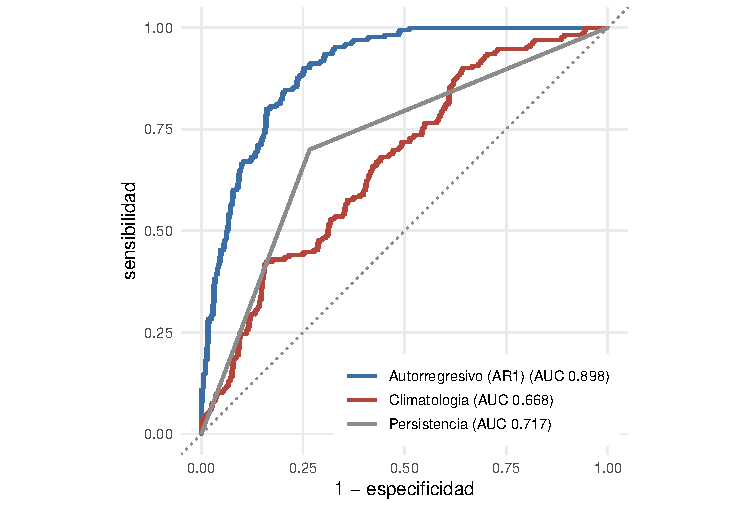
\includegraphics[width=\linewidth]{nowcast_roc.pdf}
  \caption{ROC curves in validation (2025) of the autoregressive model and
    the two baselines. Persistence produces three vertices because its
    predictor is binary.}
  \label{fig:nowcast-roc}
\end{figure}

A high AUC is not enough; it must be compared with what would be obtained
without a model. The two baselines are climatology (calendar only, AUC 0.668)
and persistence (today will be like yesterday, AUC 0.717). The model reaches
0.898 in 2025 and outperforms both with $p<10^{-5}$ in DeLong's test
(\cref{fig:nowcast-roc}). With Youden's threshold set on the fitting data
(0.327), not on the validation data, sensitivity is 0.759 and specificity
0.841: of 170 exceedance days it detects 129, with 31 false alarms in 195
clean days.

Leave-one-year-out cross-validation separates the performance on the
partition from the performance expected in an arbitrary year: the AUC ranges
from 0.840 (2021) to 0.915 (2024), with a pooled value of 0.878, 95\,\% CI
$[0.859, 0.897]$. That second figure is the generalization estimate; the
0.898 of 2025 falls within the range. The year effect is not explained by
prevalence or by station coverage, and it is the main limitation of the
model.

Two caveats bound the reading. The model underpredicts in 2025 (mean
prediction 0.338 versus 0.466 observed) because of the 2024 level step, and
it is not recalibrated because that would fit a parameter to the test
period. And it is \emph{nowcasting}, not forecasting: the factors are from
the same day as the response, so the model distinguishes days within a
season ---which climatology cannot do--- but does not anticipate tomorrow's
ozone.
